%-----------------------------------------------------------------------------%
\chapter{\babDua}
\label{bab:2}

\noindent\todo{
    kasih contoh ndcg
}

% DONE
% \noindent\todo{
%     kasih contoh recall dan presisi
% }


\section{Masalah Pemeringkatan Teks}
    \subsection{Pemeringkatan Teks}

    Permasalahan pemeringkatan teks adalah Permasalahan untuk menentukan urutan dokumen yang paling relevan dengan kueri $q$ yang diberikan. Dalam bahasa yang lebih formal, diberikan kueri $q$ dan himpunan dokumen terbatas $\mathcal{D}= \{d_1, d_2, ..., d_n\}$, keluaran yang diinginkan dari permasalahan ini adalah barisan dokumen $D_k = (d_{i_1}, d_{i_2}, ..., d_{i_k})$ yang merupakan $k$ dokumen yang paling relevan dengan kueri $q$. Selain itu, biasanya nilai $k$ akan lebih kecil dari banyaknya dokumen yang ada, sehingga permasalahan pemeringkatan sering juga disebut sebagai \f{top-k retrieval}. Untuk mengukur performa suatu model pemeringkatan, biasanya digunakan metrik evaluasi seperti presisi, \f{recall}, \f{reciprocal rank}, dan \f{normalized discounted cumulative gain} (nDCG) yang akan dijelaskan pada \sect~\ref{sec:metrik-evaluasi}. \equ~\ref{eq:top-k-retrieval}.

    \subsection{Bentuk Umum Dataset untuk Evaluasi Pemeringkatan Teks}
    \label{sec:dataset-umum}
    


        \subsubsection{\f{Judgements}}
    

    \subsection{Metrik Evaluasi dalam Pemeringkatan Teks}
    \label{sec:metrik-evaluasi}

        \subsubsection{\f{Recall} dan Presisi}

        \begin{figure}
            \centering
            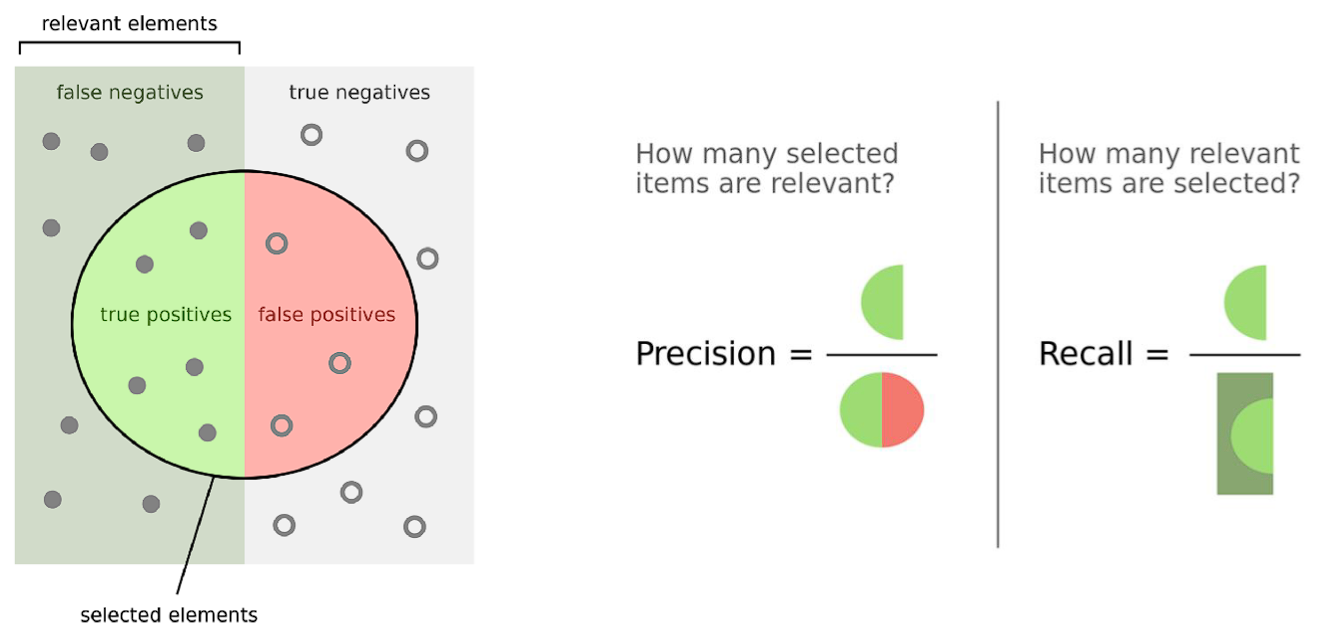
\includegraphics[width=0.50\textwidth]{assets/pics/recall-presisi.png}
            \caption{\license.}
            \label{fig:recall-precision}
        \end{figure}
        

        
        Presisi dan \f{recall} adalah metrik yang paling sederhana untuk mengukur kemampuan dari suatu model pemeringkatan teks. \f{Recall} mengukur kemampuan model untuk mengembalikan dokumen yang relevan dengan kueri $q$ dari seluruh dokumen yang relevan dengan kueri $q$ \citep{textrankingsurvey}. Di lain sisi, presisi mengukur kemampuan model dalam mengembalikan dokumen yang relevan dengan kueri $q$ dari seluruh dokumen yang dikembalikan oleh model \citep{textrankingsurvey}. Untuk suatu kueri $q$, kumpulan dokumen $\mathcal{D} = \{d_1, d_2, ..., d_n\}$, dan barisan $k$ dokumen yang diambil oleh model, $\mathcal{D}_k = (d_{i_1}, d_{i_2}, ..., d_{i_k})$, \f{recall} dan presisi dapat dihitung dengan \equ~\ref{eq:recall} dan \equ~\ref{eq:presisi}.

        \begin{align}
            \label{eq:recall}
            \mathcal{D} &= \{d_1, d_2, \dots, d_n\} \\
            D_k &= (d_{i_1}, d_{i_2}, \dots, d_{i_k}) \\
            \text{recall}(q, D_k)\text{@k} &= \frac{\sum_{d \in D_k} \text{rel}(q, d)}{\sum_{d \in \mathcal{D}} \text{rel}(q, d)} \in [0, 1] \\
            \label{eq:presisi}
            \text{precision}(q, D_k)\text{@k} &= \frac{\sum_{d \in D_k} \text{rel}(q, d)}{|D_k|} \in [0, 1] \\
            \label{eq:rel}
            \text{dengan } \text{rel}(q, d) &= \begin{cases} 
            1 & \text{jika } r > 1 \\
            0 & \text{jika } r = 0
            \end{cases}        
        \end{align}

        Sebagai Contoh, Jika terdapat 10 dokumen yang relevan dengan kueri $q$, dan model mengembalikan $k=100$ dokumen, namun hanya terdapat 5 dokumen yang relevan pada $D_k$  maka \f{recall} dan presisi dari model tersebut adalah 0.5 ($\frac{5}{10}$) dan 0.05 ($\frac{5}{100}$) masing-masing. Baik \f{recall} maupun presisi memiliki rentang nilai dari 0 hingga 1, dimana nilai 1 menunjukkan performa model yang terbaik. \pic~\ref{fig:recall-precision} mengilustrasikan metrik \f{recall} dan presisi.

        \subsubsection{\f{Reciprocal Rank}}

        \begin{figure}
            \centering
            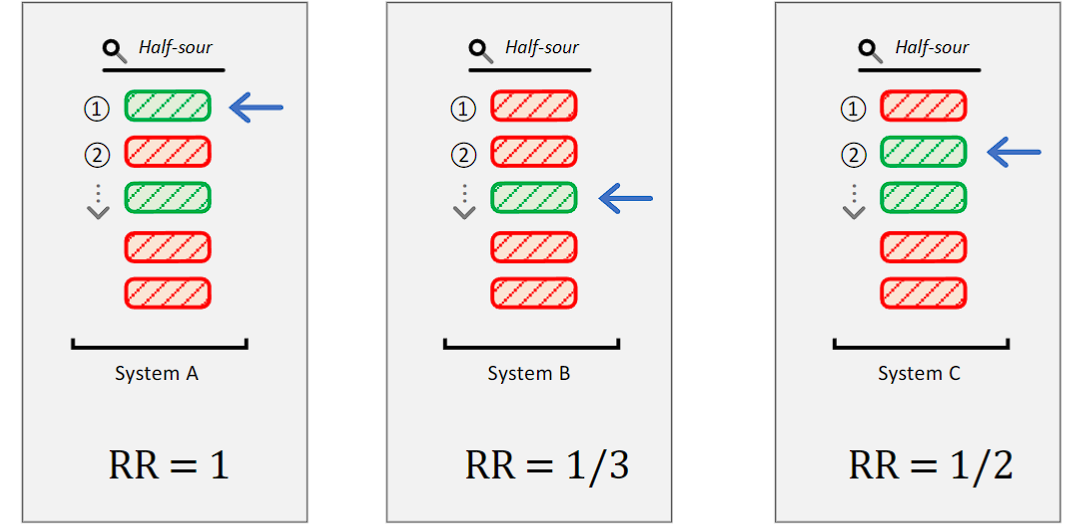
\includegraphics[width=0.50\textwidth]{assets/pics/rr.png}
            \caption{idk.}
            \label{fig:reciprocal-rank}
        \end{figure}

        Metrik lainnya yang sering digunakan untuk mengukur performa model pemeringkatan adalah \f{reciprocal rank} (RR). Metrik RR menitikberatkan pada peringkat pertama dari dokumen yang relevan dengan kueri $q$. Semakin tinggi peringkat dari dokumen yang relevan dengan kueri $q$. \equ~\ref{eq:reciprocal-rank-start} hingga \equ~\ref{eq:reciprocal-rank-end} menunjukkan cara menghitung RR dari suatu kueri $q$ dan barisan $k$ dokumen yang diambil oleh model.

        \begin{align}
            \text{RR}(q, D_k)\text{@k} &= \begin{cases}
                \label{eq:reciprocal-rank-start}
                \frac{1}{\text{FirstRank}(q, D_k)} & \text{jika } \exists d \in D_k \text{ dengan } \text{rel}(q, d) = 1 \\        
                0 & \text{jika } \forall d \in D_k, \text{ rel}(q, d) = 0 \\
                \end{cases} \in [0, 1] \\
                \label{eq:reciprocal-rank-end}
                \text{FirstRank}(q,D_k) &= \text{posisi dokumen relevan pertama } d\in D_k \text{ dengan } \text{rel}(q, d) = 1
        \end{align}

        \pic~\ref{fig:reciprocal-rank} mengilustrasikan metrik RR. Pada gambar tersebut, nilai RR dari sistem A adalah 1 $(\frac{1}{1})$ karena posisi dari dokumen yang relevan pertama adalah 1. Sedangkan nilai RR dari sistem B dan sistem C masing-masing adalah  0.33 $(\frac{1}{3})$ dan 0.5 $(\frac{1}{2})$ karena posisi dari dokumen yang relevan pertama adalah 3 dan 2. Selain itu, jika tidak terdapat dokumen yang relevan dengan kueri $q$ pada $D_k$, maka nilai RR dari sistem tersebut adalah 0. 

        \subsubsection{\f{Normalized Discounted Cumulative Gain} (nDCG)}
        \f{Normalized Discounted Cumulative Gain} (nDCG) adalah metrik yang umumnya digunakan untuk mengukur kualitas dari pencarian situs web. Tidak seperti metrik yang telah disebutkan sebelumnya, nDCG dirancang untuk suatu \f{judgements} $r$ yang tak biner. Fungsi $\text{rel}(q, d)$ pada \equ~\ref{eq:rel} berubah menjadi $\text{rel(q,d)}  = r $ ketika menghitung metrik nDCG. \equ~\ref{eq:ndcg-start} hingga \equ~\ref{eq:ndcg-end} menunjukkan cara menghitung nDCG dari suatu kueri $q$ dan barisan $k$ dokumen yang diambil oleh model.

        \begin{align}
            \label{eq:ndcg-start}
            \text{nDCG}(q, D_k)\text{@k} &= \frac{\text{DCG}(q, D_k)\text{@k}}{\text{DCG}(q, D_k^{\text{ideal}})\text{@k}} \in [0, 1] \\
            \label{eq:dcg}
            \text{DCG}(q, D_k)\text{@k} &= \sum_{d \in D_k} \frac{2^{\text{rel}(q, d)} - 1}{\log_2(\text{rank}(d, D_k) + 1)} \\
            \label{eq:ndcg-end}
            \text{rank}(d,D_k) &= \text{Posisi } d \text{ dalam } D_k \\
            \text{rel}(q, d) &= r
        \end{align}

        Perhitungan \f{discounted cumulative gain} (DCG) pada \equ~\ref{eq:dcg} dapat dijelaskan menjadi dua faktor, yaitu:
        \begin{enumerate}
            \item faktor $2^{\text{rel}(q, d)} - 1$ menunjukkan bahwa dokumen yang lebih relevan akan memiliki nilai yang lebih tinggi dari dokumen yang kurang relevan.
            \item faktor $\frac{1}{\log_2(\text{rank}(d, D_k) + 1)}$ menunjukkan bahwa dokumen yang relevan yang muncul pada peringkat yang lebih tinggi akan memiliki nilai yang lebih tinggi dari dokumen dengan relevansi yang sama, tetapi muncul pada peringkat yang lebih rendah.
        \end{enumerate}

        nilai dari nDCG pada \equ~\ref{eq:ndcg-start} adalah nilai DCG pada barisan dokumen $D_k$ yang dinormalisasi oleh nilai DCG pada barisan dokumen ideal $D_k^{\text{ideal}}$. Barisan dokumen ideal $D_k^{\text{ideal}}$ adalah barisan dokumen yang diurutkan berdasarkan relevansinya dengan kueri $q$.

        Biasanya, metrik nDCG digunakan untuk \f{dataset} dengan \f{judgements} $r$ yang padat. Selain itu, jika pada \f{datasets} memiliki \f{judgements} biner, faktor $2^{\text{rel}(q, d)} - 1$ pada \equ~\ref{eq:dcg} dapat diubah menjadi $\text{rel}(q, d)$. \equ~\ref{eq:dcg} akan menjadi \equ~\ref{eq:dcg-binary}.
        
        \begin{align}
        \label{eq:dcg-binary}
        \text{DCG}(q, D_k)\text{@k} &= \sum_{d \in D_k} \frac{\text{rel}(q, d)}{\log_2(\text{rank}(d, D_k) + 1)}.
        \end{align}


\section{Pemeringkatan Teks dengan Statistik}

    \subsection{\f{Term Frequency - Inverse Document Frequency} (TF-IDF)}
    \subsection{\f{Best Match 25} (BM25)}


\section{Arsitektur \f{Deep Learning}}

    \subsection{\f{Multilayer Perceptron} (MLP)}

    \subsection{Fungsi Aktivasi}

    \subsection{Fungsi \f{Loss}}
        
    \subsection{\f{Backpropagation}}

    \subsection{Inisialisasi Bobot}
        \subsubsection{Inisialisasi Kaiming Menjaga Variansi \f{ouput} pada \f{Hidden Layer}}

        \subsubsection{Insialisasi Kaiming Menjaga Variansi Gradien}



\section{Pembelajaran Representasi}

    \subsection{Fungsi \f{Loss} pada Pembelajaran Representasi}













        

